\documentclass[12pt]{report}
\usepackage[utf8]{inputenc}
\usepackage[russian]{babel}
%\usepackage[14pt]{extsizes}
\usepackage{listings}
\usepackage{graphicx}
\usepackage{amsmath,amsfonts,amssymb,amsthm,mathtools} 
\usepackage{pgfplots}
\usepackage{filecontents}
\usepackage{float}
\usepackage{indentfirst}
\usepackage{eucal}
\usepackage{enumitem}
\frenchspacing

\usepackage{indentfirst} % Красная строка


\usetikzlibrary{datavisualization}
\usetikzlibrary{datavisualization.formats.functions}

\usepackage{amsmath}




% Для листинга кода:
\lstset{ %
language=haskell,                 % выбор языка для подсветки (здесь это С)
basicstyle=\small\sffamily, % размер и начертание шрифта для подсветки кода
numbers=left,               % где поставить нумерацию строк (слева\справа)
numberstyle=\tiny,           % размер шрифта для номеров строк
stepnumber=1,                   % размер шага между двумя номерами строк
numbersep=5pt,                % как далеко отстоят номера строк от подсвечиваемого кода
showspaces=false,            % показывать или нет пробелы специальными отступами
showstringspaces=false,      % показывать или нет пробелы в строках
showtabs=false,             % показывать или нет табуляцию в строках
frame=single,              % рисовать рамку вокруг кода
tabsize=2,                 % размер табуляции по умолчанию равен 2 пробелам
captionpos=t,              % позиция заголовка вверху [t] или внизу [b] 
breaklines=true,           % автоматически переносить строки (да\нет)
breakatwhitespace=false, % переносить строки только если есть пробел
escapeinside={\#*}{*)}   % если нужно добавить комментарии в коде
}

\usepackage[left=2cm,right=2cm, top=2cm,bottom=2cm,bindingoffset=0cm]{geometry}
% Для измененных титулов глав:
\usepackage{titlesec, blindtext, color} % подключаем нужные пакеты
\definecolor{gray75}{gray}{0.75} % определяем цвет
\newcommand{\hsp}{\hspace{20pt}} % длина линии в 20pt
% titleformat определяет стиль
\titleformat{\chapter}[hang]{\Huge\bfseries}{\thechapter\hsp\textcolor{gray75}{|}\hsp}{0pt}{\Huge\bfseries}


% plot
\usepackage{pgfplots}
\usepackage{filecontents}
\usetikzlibrary{datavisualization}
\usetikzlibrary{datavisualization.formats.functions}

\begin{document}
%\def\chaptername{} % убирает "Глава"
\thispagestyle{empty}
\begin{titlepage}
	\noindent \begin{minipage}{0.15\textwidth}
	
\includegraphics[width=\linewidth]{b_logo}
	\end{minipage}
	\noindent\begin{minipage}{0.9\textwidth}\centering
		\textbf{Министерство науки и высшего образования Российской Федерации}\\
		\textbf{Федеральное государственное бюджетное образовательное учреждение высшего образования}\\
		\textbf{~~~«Московский государственный технический университет имени Н.Э.~Баумана}\\
		\textbf{(национальный исследовательский университет)»}\\
		\textbf{(МГТУ им. Н.Э.~Баумана)}
	\end{minipage}
	
	\noindent\rule{18cm}{3pt}
	\newline\newline
	\noindent ФАКУЛЬТЕТ $\underline{\text{«Информатика и системы управления»}}$ \newline\newline
	\noindent КАФЕДРА $\underline{\text{«Программное обеспечение ЭВМ и информационные технологии»}}$\newline\newline\newline\newline\newline
	
	
	\begin{center}
		\noindent\begin{minipage}{1.3\textwidth}\centering
			\Large\textbf{  Отчет по лабораторной работе №4}\newline
			\textbf{по дисциплине "Операционные системы"}\newline\newline
		\end{minipage}
	\end{center}
	
	\noindent\textbf{Тема} $\underline{\text{Процессы. Системные вызовы fork() и exec()}}$\newline\newline
	\noindent\textbf{Студент} $\underline{\text{Варламова Е. А. ~~~~~~~~~~~~~~~~~~~~~~~~~~~~~~~~~}}$\newline\newline
	\noindent\textbf{Группа} $\underline{\text{ИУ7-51Б~~~~~~~~~~~~~~~~~~~~~~~~~~~~~~~~~~~~~~~~~~~~~~}}$\newline\newline
	\noindent\textbf{Оценка (баллы)} $\underline{\text{~~~~~~~~~~~~~~~~~~~~~~~~~~~~~~~~~~~~~~~~~~~~~}}$\newline\newline
	\noindent\textbf{Преподаватели} $\underline{\text{Рязанова Н. Ю.~~~~~~~~~~~~~~~~~~~~~~~~~}}$\newline\newline\newline
	
	\begin{center}
		\vfill
		Москва~---~\the\year
		~г.
	\end{center}
\end{titlepage}

\newpage

\section*{Задание №1}

Процессы-сироты. В программе создаются не менее двух потомков системным вызовом fork(). В потомках вызывается sleep(), чтобы предок гарантированно завершился раньше своих потомков. В предке вывести собственный идентификатор, идентификатор группы и идентификаторы потомков. В процессе-потомке вывести собственный идентификатор, идентификатор предка и идентификатор группы. Убедиться, что при завершении процесса-предка потомок, который продолжает выполняться, получает идентификатор предка (PPID), равный 1 или идентификатор процесса-посредника. Продемонстрировать с помощью соответствующего вывода информацию об идентификаторах процессов и их группе. Продемонстрировать «усыновление». Для этого надо в потомках вывести идентификаторы: собственный, предка, группы до блокировки и после блокировки.

В программе добавлен sleep в предке перед его завершением для того, чтобы предок не завершился до того, как будет выведена информация о процессах-потомках до блокировки. При этом время блокировки предка меньше, чем время блокировки потомков, поэтому предок гарантированно завершится раньше своих потомков.

Текст программы приведён на листинге \ref{task01:prog}.

\begin{lstlisting}[label=task01:prog,caption=Процессы-сироты,language=C]
#include <stdio.h>
#include <unistd.h>
#define ERROR_FORK 1
#define OK 0
int main() {
    int childpids[2];
    for (int i = 0; i < 2; i++) {
        int pid = fork();

        if (pid == -1) {
            return ERROR_FORK;
        }

        if (pid == 0) {
            printf("\nCHILD №%d BEFORE BLOCK: pid: %d, ppid: %d, grp: %d\n", i + 1, getpid(), getppid(), getpgrp());
            sleep(2);
            printf("\nCHILD №%d AFTER BLOCK: pid: %d, ppid: %d, grp: %d\n", i + 1, getpid(), getppid(), getpgrp());
            return OK;
        }

        childpids[i] = pid;
    }
    printf("PARENT: pid: %d grp: %d, child's pids: %d, %d\n", getpid(), getpgrp(), childpids[0], childpids[1]);
    sleep(1);
    return OK;
}
\end{lstlisting}

На риснуке \ref{task01:demo} приведён результат работы программы. Видно, что до завершения процесса-предка ppid у потомков был равен идентификатору предка. Затем, когда процесс-предок завершился, потомки были "усыновлены" процессом с идентификатором 1.  
\begin{figure}[H]

	\centering

	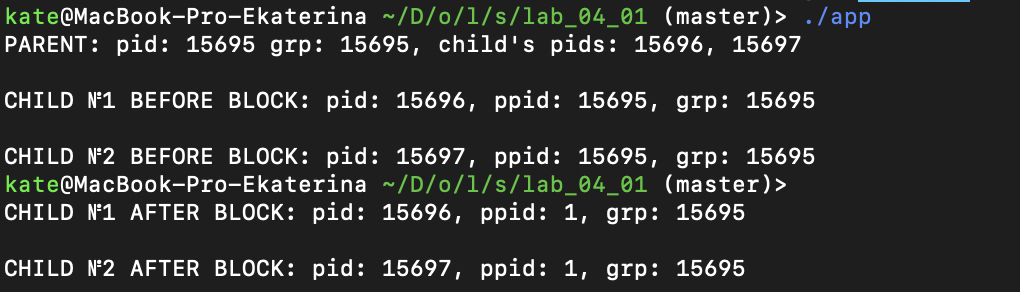
\includegraphics[width=\linewidth]{task01.png}
	\caption{Демонстрация работы программы (задание №1).}

	\label{task01:demo}

\end{figure}
\newpage
\section*{Задание №2}

Предок ждет завершения своих потомком, используя системный вызов wait(). Вывод соответствующих сообщений на экран. В программе необходимо, чтобы предок выполнял анализ кодов завершения потомков. Текст программы приведён на листинге \ref{task02:prog}.

\begin{lstlisting}[label=task02:prog,caption=Системный вызов wait(),language=C]
#include <stdio.h>
#include <unistd.h>
#include <sys/types.h>
#include <sys/wait.h>
#define ERROR_FORK 1
#define OK 0
int main() {
    int childpids[2];
    for (int i = 0; i < 2; i++) {
        int pid = fork();
        if (pid == -1) {
            return ERROR_FORK;
        }
        if (pid == 0){
            sleep(2);
            printf("CHILD №%d: pid: %d, ppid: %d, grp: %d\n", i + 1, getpid(), getppid(), getpgrp());
            return OK;
        }
        childpids[i] = pid;
    }
    printf("PARENT: pid: %d grp: %d, child's pids: %d, %d\n", getpid(), getpgrp(), childpids[0], childpids[1]);
    for (int i = 0; i < 2; i++)
    {
        int status;
        pid_t childpid = wait(&status);
        if (WIFEXITED(status)) {
            printf("PARENT: child №%d (PID = %d) has finished with code: %d\n", i + 1, childpid, WEXITSTATUS(status));
        }
        else if (WIFSIGNALED(status)) {
            printf("PARENT: child №%d (PID = %d) has finished because of signal: %d\n", i + 1, childpid, WTERMSIG(status));
        }
        else if (WIFSTOPPED(status)) {
            printf("PARENT: child №%d (PID = %d) has been stopped because of signal: %d\n", i + 1, childpid, WSTOPSIG(status));
        }
    }
    return OK;
}
\end{lstlisting}

Результат работы программы приведён на рисунке \ref{task02:demo}. Видно, что в отличие от программы из первого задания процесс-предок дождался завершения дочерних процессов, о чём свидетельствуют коды завершения дочерних процессов, перехваченные процессом-предком.
\begin{figure}[H]
	\centering
	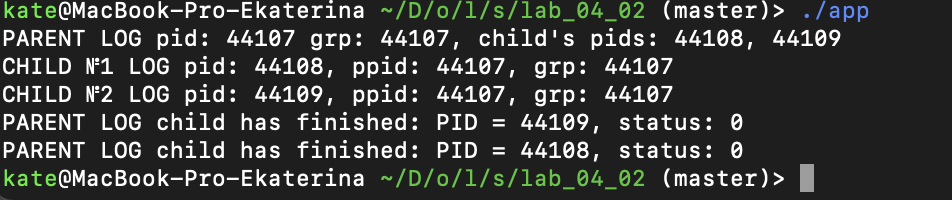
\includegraphics[width=\linewidth]{task02.png}
	\caption{Демонстрация работы программы (задание №2).}
	\label{task02:demo}
\end{figure}

\newpage
\section*{Задание №3}

Потомки переходят на выполнение других программ, которые передаются системному вызову exec() в качестве параметра. Потомки должны выполнять разные программы. Предок ждет завершения своих потомков с анализом кодов завершения. На экран выводятся соответствующие сообщения. Текст программы приведён на листинге \ref{task03:prog}.

\begin{lstlisting}[label=task03:prog,caption=Системный вызов exec(),language=C]
#include <stdio.h>
#include <unistd.h>
#include <sys/types.h>
#include <sys/wait.h>
#define ERROR_FORK 1
#define ERROR_EXEC 2
#define OK 0
int main() {
    int childpids[2];
    for (int i = 0; i < 2; i++) {
        int pid = fork();
        if (pid == -1) {
            return ERROR_FORK;
        }
        if (pid == 0) {
            printf("CHILD №%d: pid: %d, ppid: %d, grp: %d\n", i + 1, getpid(), getppid(), getpgrp());
            if (i == 0) execl("sort", "sort", "1", "3", "2", "0", "4", "5", NULL);
            else execl("max", "max", "1", "3", "2", "0", "4", "5", NULL);
            return ERROR_EXEC;
        }
        childpids[i] = pid;
    }
    printf("PARENT: pid: %d grp: %d, child's pids: %d, %d\n", getpid(), getpgrp(), childpids[0], childpids[1]);
    for (int i = 0; i < 2; i++) {
        int status;
        pid_t childpid = wait(&status);
        if (WIFEXITED(status)) {
            printf("PARENT: child №%d (PID = %d) has finished with code: %d\n", i + 1, childpid, WEXITSTATUS(status));
        } else if (WIFSIGNALED(status)) {
            printf("PARENT: child №%d (PID = %d) has finished because of signal: %d\n", i + 1, childpid, WTERMSIG(status));
        } else if (WIFSTOPPED(status)) {
            printf("PARENT: child №%d (PID = %d) has been stopped because of signal: %d\n", i + 1, childpid, WSTOPSIG(status));
        }
    }
    return OK; }
\end{lstlisting}

Результат работы программы приведён на рисунке \ref{task03:demo}. Видно, что в отличие от программы из второго задания дочерние процессы переходят на выполнение других программ, которые передаются системному вызову exec() в качестве параметра. В данном случае выполняются программы "sort" и "max" с аргументами в виде элементов обрабатываемого массива (массив: [1, 3, 2, 0, 4, 5]). Программа sort выводит отсортированный массив, программа max выводит максимальный элемент в массиве. Исходные коды программ сортировки и поиска максимума приведены в приложениях в листингах \ref{sort} и \ref{max} соответственно.
\begin{figure}[H]
	\centering
	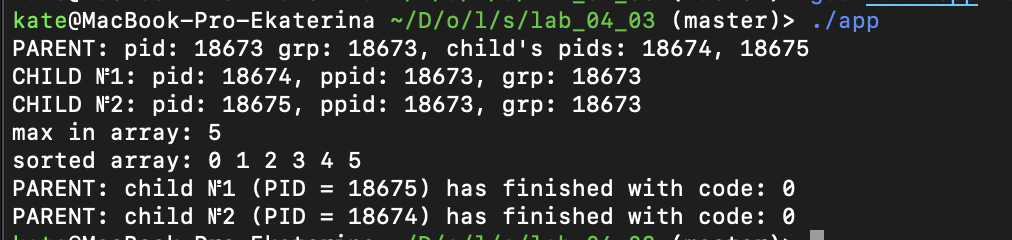
\includegraphics[width=\linewidth]{task03.png}
	\caption{Демонстрация работы программы (задание №3).}
	\label{task03:demo}

\end{figure}
\newpage
\section*{Задание №4}

Предок и потомки обмениваются сообщениями через неименованный программный канал. Причем оба потомка пишут свои сообщения в один программный канал, а предок их считывает из канала. Потомки должны посылать предку разные сообщения по содержанию и размеру. Предок считывает сообщения от потомков и выводит их на экран. Предок ждет завершения своих потомков и анализирует код их завершения. Вывод соответствующих сообщений на экран. Текст программы приведён на листинге \ref{task04:prog}.

\begin{lstlisting}[label=task04:prog,caption=Программные каналы,language=C]
#include <stdio.h>
#include <unistd.h>
#include <sys/types.h>
#include <sys/wait.h>
#include "string"
#define ERROR_FORK 1
#define ERROR_EXEC 2
#define ERROR_PIPE 3
#define OK 0
int main() {
    int fd[2];
    const char *messages[2] = { "msg\n", "msg msg\n"};
    if (pipe(fd) == -1) {
        return ERROR_PIPE;
    }
    int childpids[2];
    for (int i = 0; i < 2; i++) {
        int pid = fork();
        if (pid == -1) {
            return ERROR_FORK;
        }

        if (pid == 0) {
            close(fd[0]);
            write(fd[1], messages[i], strlen(messages[i]));
            printf("CHILD №%d (pid: %d, ppid: %d, grp: %d) sent message to parent\n", i + 1, getpid(), getppid(), getpgrp());
            return OK;
        }
        childpids[i] = pid;
    }
    printf("PARENT: pid: %d grp: %d, child's pids: %d, %d\n", getpid(), getpgrp(), childpids[0], childpids[1]);
    for (int i = 0; i < 2; i++) {
        int status;
        pid_t childpid = wait(&status);
        if (WIFEXITED(status)) {
            printf("PARENT: child №%d (PID = %d) has finished with code: %d\n", i + 1, childpid, WEXITSTATUS(status));
        } else if (WIFSIGNALED(status)) {
            printf("PARENT: child №%d (PID = %d) has finished because of signal: %d\n", i + 1, childpid, WTERMSIG(status));
        } else if (WIFSTOPPED(status)) {
            printf("PARENT: child №%d (PID = %d) has been stopped because of signal: %d\n", i + 1, childpid, WSTOPSIG(status));
        }
    }
    char buf[15];
    close(fd[1]);
    read(fd[0], buf, 15);
    printf("PARENT: received messages:\n%s", buf);
    return OK;
}
\end{lstlisting}

Результат работы программы приведён на рисунке \ref{task04:demo}. 
\begin{figure}[H]

	\centering

	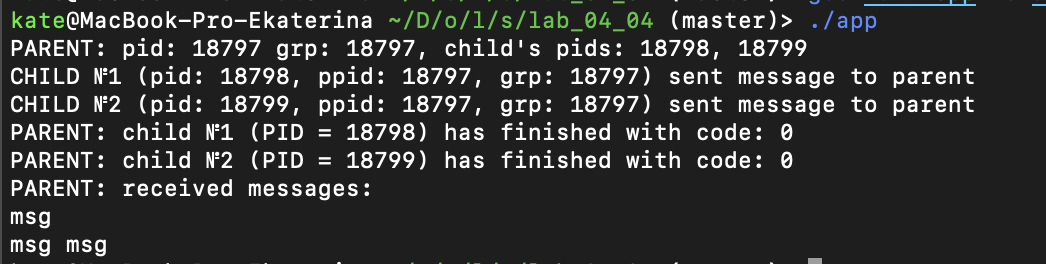
\includegraphics[width=\linewidth]{task04.png}
	\caption{Демонстрация работы программы (задание №4).}

	\label{task04:demo}

\end{figure}
\newpage
\section*{Задание №5}
Предок и потомки обмениваются сообщениями через неименованный программный канал. В программу включается собственный обработчик сигнала. С помощью сигнала меняется ход выполнения программы. При получении сигнала потомки записывают сообщения в канал, если сигнал не поступает, то не записывают. Предок ждет завершения своих потомков и анализирует коды их завершений. Вывод соответствующих сообщений на экран. Вывод соответствующих сообщений на экран. Текст программы приведён на листинге \ref{task05:prog}.

\begin{lstlisting}[label=task05:prog,caption=Использование сигналов,language=C]
#include <stdio.h>
#include <unistd.h>
#include <sys/types.h>
#include <sys/wait.h>
#include "string"
#define ERROR_FORK 1
#define ERROR_EXEC 2
#define ERROR_PIPE 3
#define OK 0
bool sendSig = 0;
void empty(int sig){ }
void sendSigSwitch(int sig) {
    sendSig = 1;
}
int main() {
    signal(SIGINT, empty);
    int fd[2];
    const char *messages[2] = { "msg\n", "msg msg\n"};
    if (pipe(fd) == -1) {
        return ERROR_PIPE;
    }
    int childpids[2];
    for (int i = 0; i < 2; i++) {
        int pid = fork();
        if (pid == -1) {
            return ERROR_FORK;
        }
        if (pid == 0) {
            signal(SIGINT, sendSigSwitch);
            sleep(4);
            if (sendSig) {
                close(fd[0]);
                write(fd[1], messages[i], strlen(messages[i]));
                printf("CHILD №%d: (pid: %d, ppid: %d, grp: %d) sent message to parent\n", i + 1, getpid(), getppid(), getpgrp());
            }
            else {
                printf("CHILD №%d: didn't send a message\n", i + 1);
            }
            return OK;
        }
        childpids[i] = pid;
    }
    printf("PARENT: pid: %d grp: %d, child's pids: %d, %d\n", getpid(), getpgrp(), childpids[0], childpids[1]);
    for (int i = 0; i < 2; i++) {
        int status;
        pid_t childpid = wait(&status);
        if (WIFEXITED(status)) {
            printf("PARENT: child №%d (PID = %d) has finished with code: %d\n", i + 1, childpid, WEXITSTATUS(status));
        }
        else if (WIFSIGNALED(status)) {
            printf("PARENT: child №%d (PID = %d) has finished because of signal: %d\n", i + 1, childpid, WTERMSIG(status));
        }
        else if (WIFSTOPPED(status)) {
            printf("PARENT: child №%d (PID = %d) has been stopped because of signal: %d\n", i + 1, childpid, WSTOPSIG(status));
        }
    }
    char buf[15];
    close(fd[1]);
    read(fd[0], buf, 15);
    printf("PARENT: received messages:\n%s", buf);
    return OK;
}
\end{lstlisting}
\newpage
Результат работы программы приведён на рисунке \ref{task05:demo}. При первом запуске был испущен сигнал SIGINT, при втором не был.
\begin{figure}[H]
	\centering
	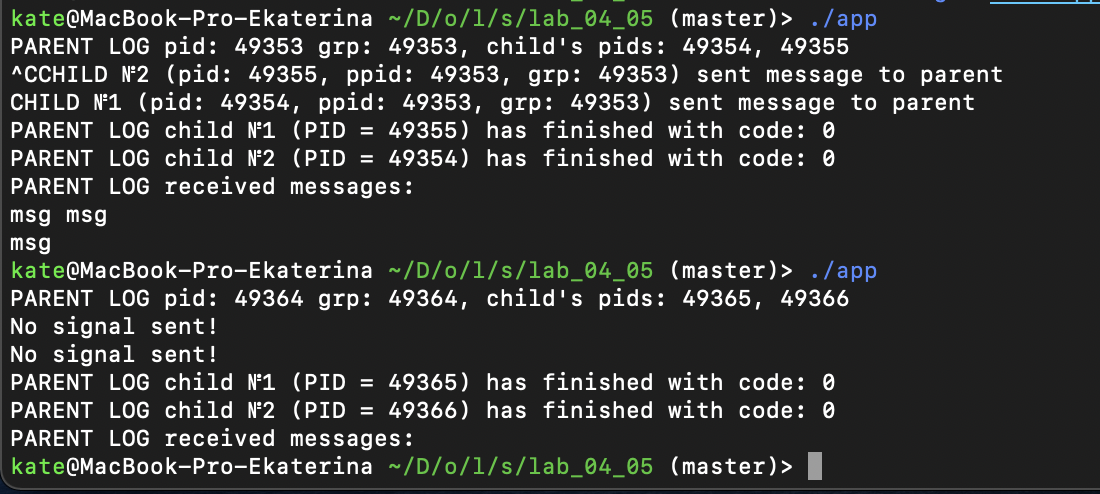
\includegraphics[width=\linewidth]{task05.png}
	\caption{Демонстрация работы программы (задание №5).}
	\label{task05:demo}
\end{figure}

\newpage
\section*{Дополнительное задание}
\begin{figure}[H]
	\centering
	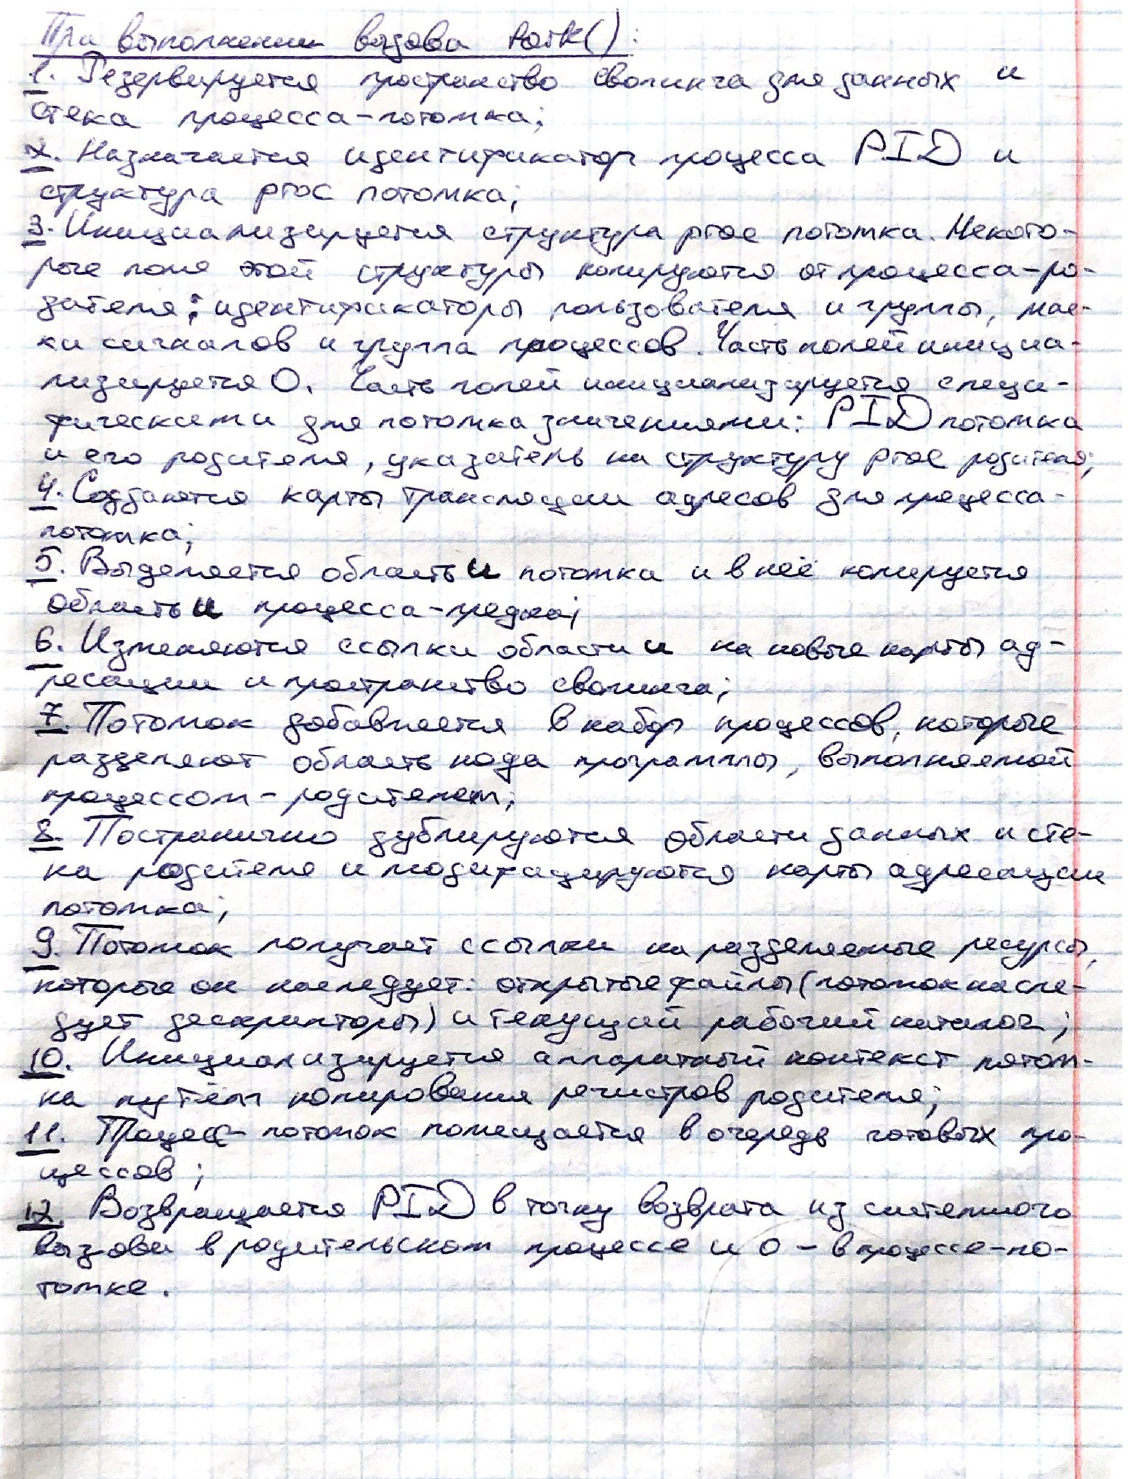
\includegraphics[scale = 0.8]{1.jpg}
	\caption{Последовательность действий fork}
	\label{task05:demo}
\end{figure}
\begin{figure}[H]
	\centering
	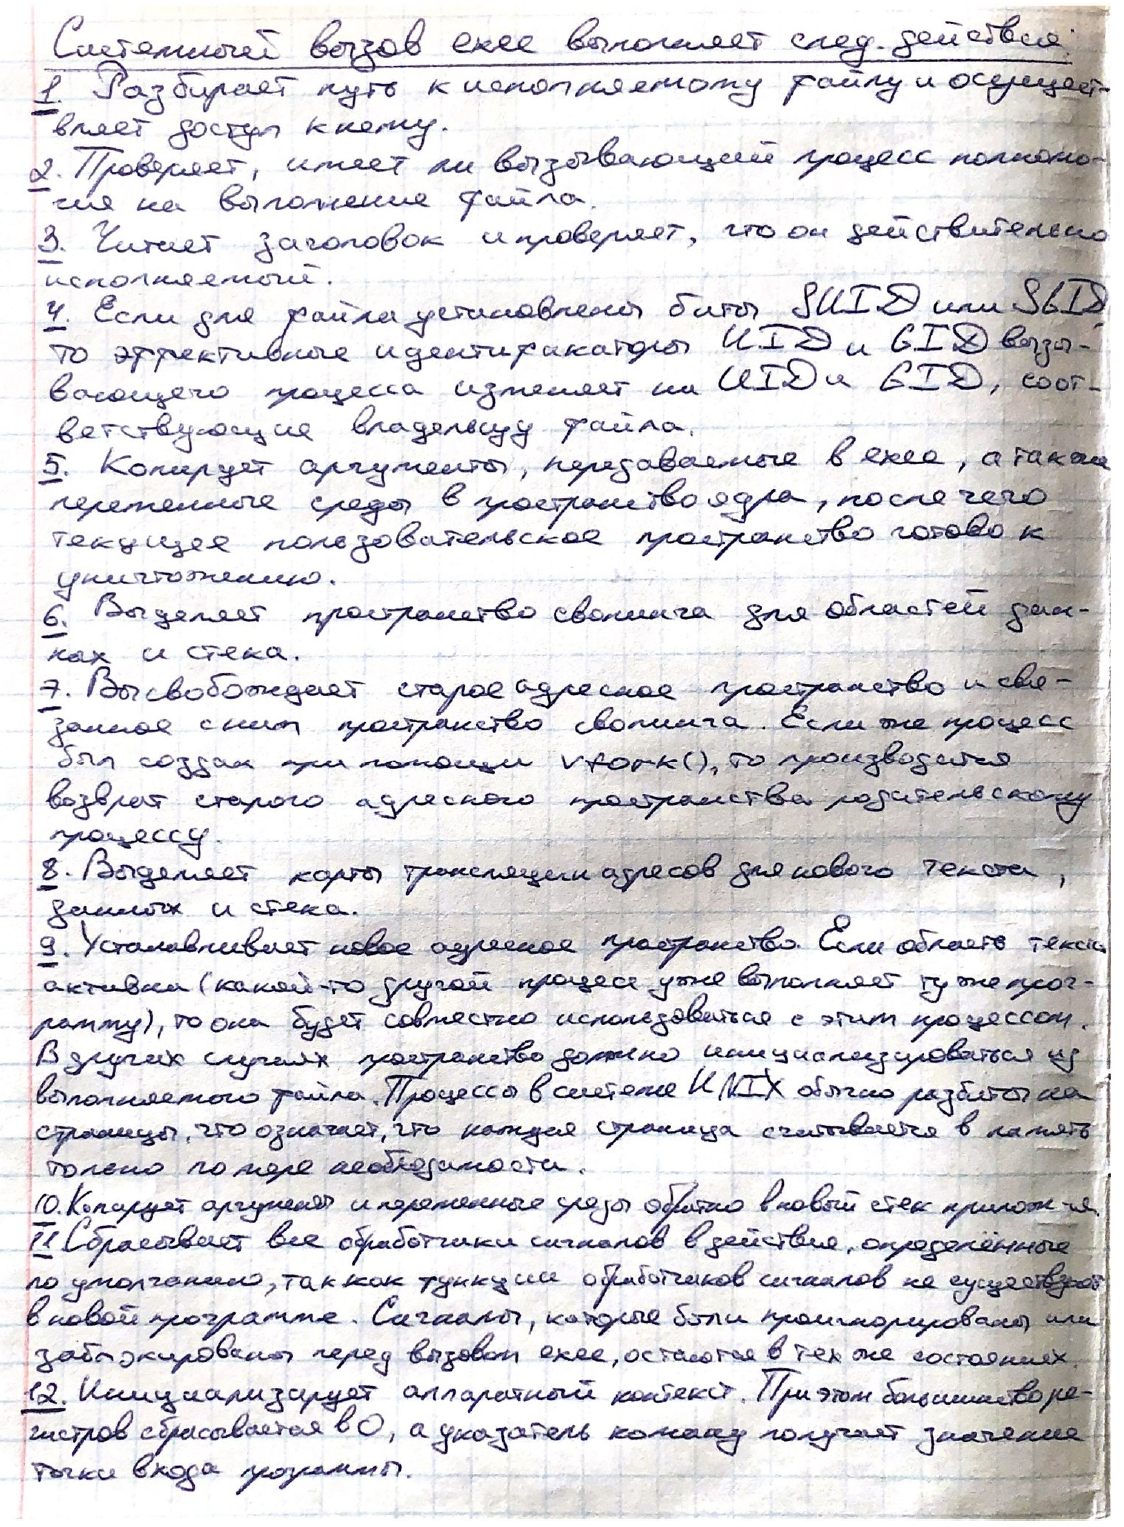
\includegraphics[scale = 0.8]{2.jpg}
	\caption{Последовательность действий exec}
	\label{task05:demo}
\end{figure}

\newpage
\section*{Приложения}
\begin{lstlisting}[label=sort,caption=Сортировка,language=C]
#include <iostream>
#define ERROR 1
void swap(char *p1, char *p2, size_t size)
{
    if (!size || !p1 || !p1)
        return;
    char q;
    for (size_t i = 0; i < size; i++)
    {
        q = *p1;
        *p1 = *p2;
        *p2 = q;
        p1++;
        p2++;
    }
}
void sort(void *beg, size_t number, size_t size, int (*comparator)(const void *, const void *))
{
    if (beg == NULL || comparator == NULL)
        return;
    char *pb = (char *)beg;
    char *pe = pb + size * number;
    if (pb == pe)
        return;
    pe -= size;
    char *ptr = NULL, *max_ptr = NULL;
    while (pe > pb)
    {
        max_ptr = ptr = pe;
        while (ptr >= pb)
        {
            if (comparator(ptr, max_ptr) > 0)
                max_ptr = ptr;
            ptr -= size;
        }
        if (max_ptr != pe)
            swap(max_ptr, pe, size);
        pe -= size;
    }
    return;
}
int compare_int(const void *f, const void *s)
{
    int *a = (int *)(f);
    int *b = (int *)(s);
    return *a - *b;
}
int main(int argc, const char *argv[])
{
    if (argc - 1 <= 0)
        return ERROR;
    int *a = (int *)malloc((argc - 1) * sizeof(int));
    if (a == NULL)
        return ERROR;
    for (int i = 1; i < argc; i++)
        a[i - 1] = atoi(argv[i]);

    sort(a, argc - 1, sizeof (int), compare_int);

    printf("sorted array: ");
    for (int i = 0; i < argc - 1; i++)
        printf("%d ", a[i]);
    printf("\n");
    free(a);
    return 0;
}
\end{lstlisting}
\begin{lstlisting}[label=max,caption=Поиск максимума,language=C]
#include <stdio.h>
#include <cstdlib>
#define ERROR 1
int main(int argc, const char *argv[])
{
    if (argc < 2)
        return ERROR;
    int max = atoi(argv[1]), tmp;
    for (int i = 2; i < argc; i++)
        if ((tmp = atoi(argv[i])) > max)
            max = tmp;
    printf("max in array: %d\n", max);
    return 0;
}

\end{lstlisting}

\end{document}